\documentclass[UKenglish, aspectratio = 169]{beamer}


\usetheme{SUT}
\usepackage{style}
\usepackage{transparent}
\usepackage{caption}
%\usepackage{xepersian}
\captionsetup[figure]{labelformat=empty}

\author[Author Name]
{FirstName LastName\\Sharif University of Technology\\author@email.com}
\title{Optimization of Real Time ddPCR \\using Deep Learning}
\subtitle{A presentation template}

\begin{document}
     \begin{frame}[allowframebreaks]
% if the TOC does not fit one frame.
%\begin{frame}{Table of contents}
    \tableofcontents
\end{frame}

\section{Introduction}
	\subsection{PCR}
	\subsection{Literature Review}
\section{Current Status}
	\subsection{Optical Subsystem}
	\subsection{Computational Subsystem}
\section{Future Steps}
\section{Conclusion}
	
\begin{frame}{What is PCR}
		\begin{figure}
			\vspace{0.5cm}
			\begin{itemize}
					\item Polymerase Chain Reaction is a chemical reaction widely used for creating copies from a specific DNA sequence for diagnosis and forensic applications.
				\end{itemize}
			\centering
			\vspace{0.2cm}
			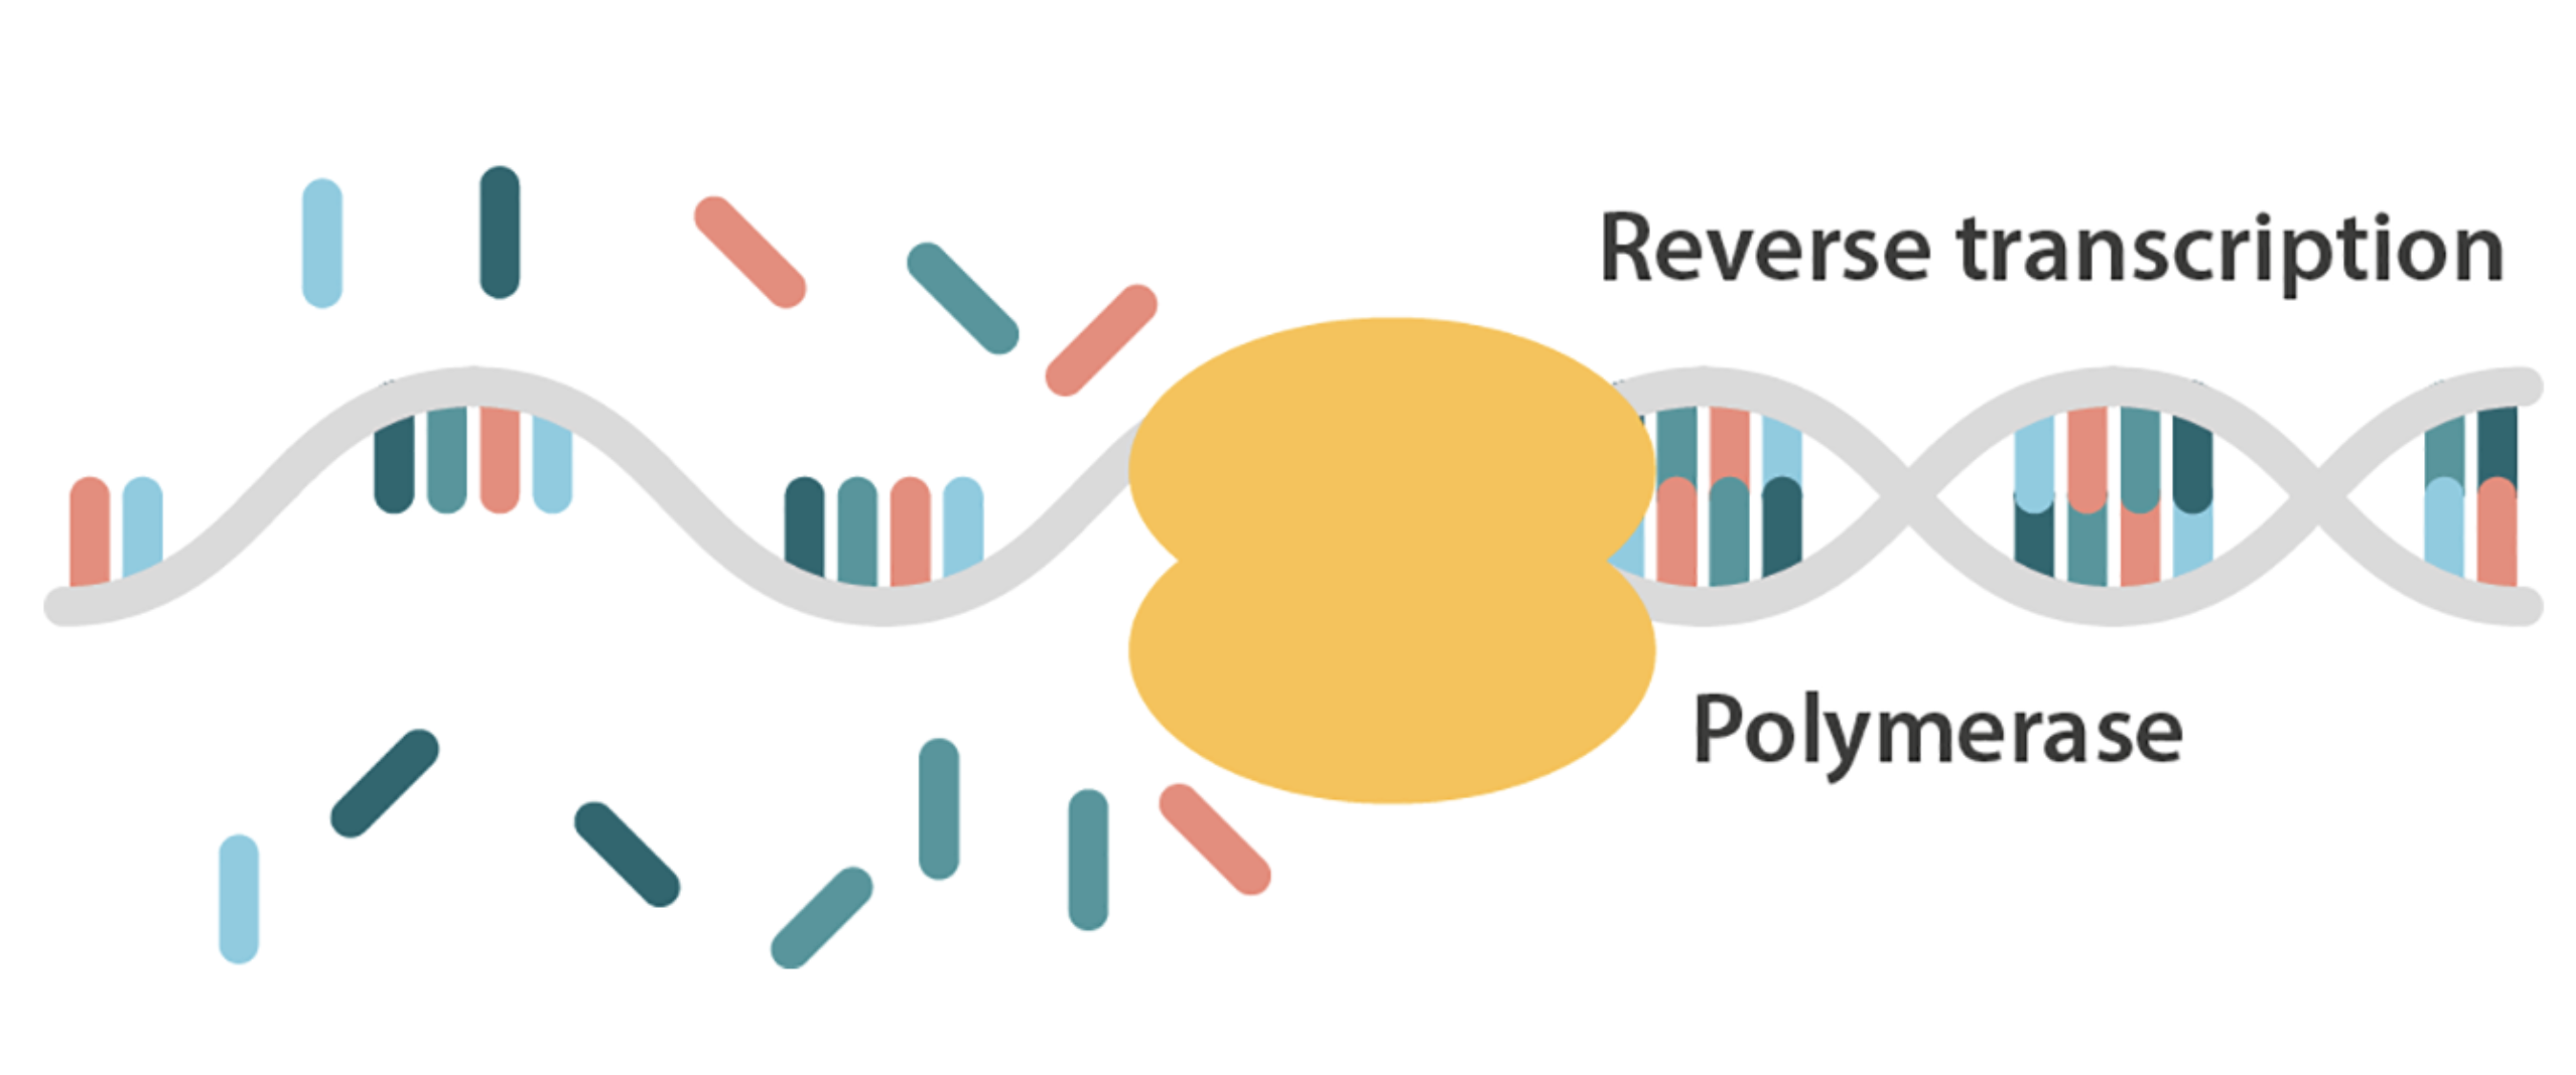
\includegraphics[scale = 0.20]{OM-images/PCR.png}
			\caption{\tiny{IAEA Bulletin, Infectious Diseases, June 2020}}
		\end{figure}
\end{frame}

\begin{frame}{PCR Cycle}
	\setbeamercovered{transparent=35}
	\begin{columns}
		\begin{column}{0.4\textwidth}
			\begin{enumerate}[<+->]
				\item<1-> Denaturation in $90^\circ C-95^\circ C$
				\item<2-> Annealing in $65^\circ C-68^\circ C$
				\item<3-> Extension in $72^\circ C$
			\end{enumerate}
		\end{column}
			\begin{column}{0.6\textwidth}
				\onslide<1->
		\begin{figure}
			\centering
			\parbox{\linewidth}{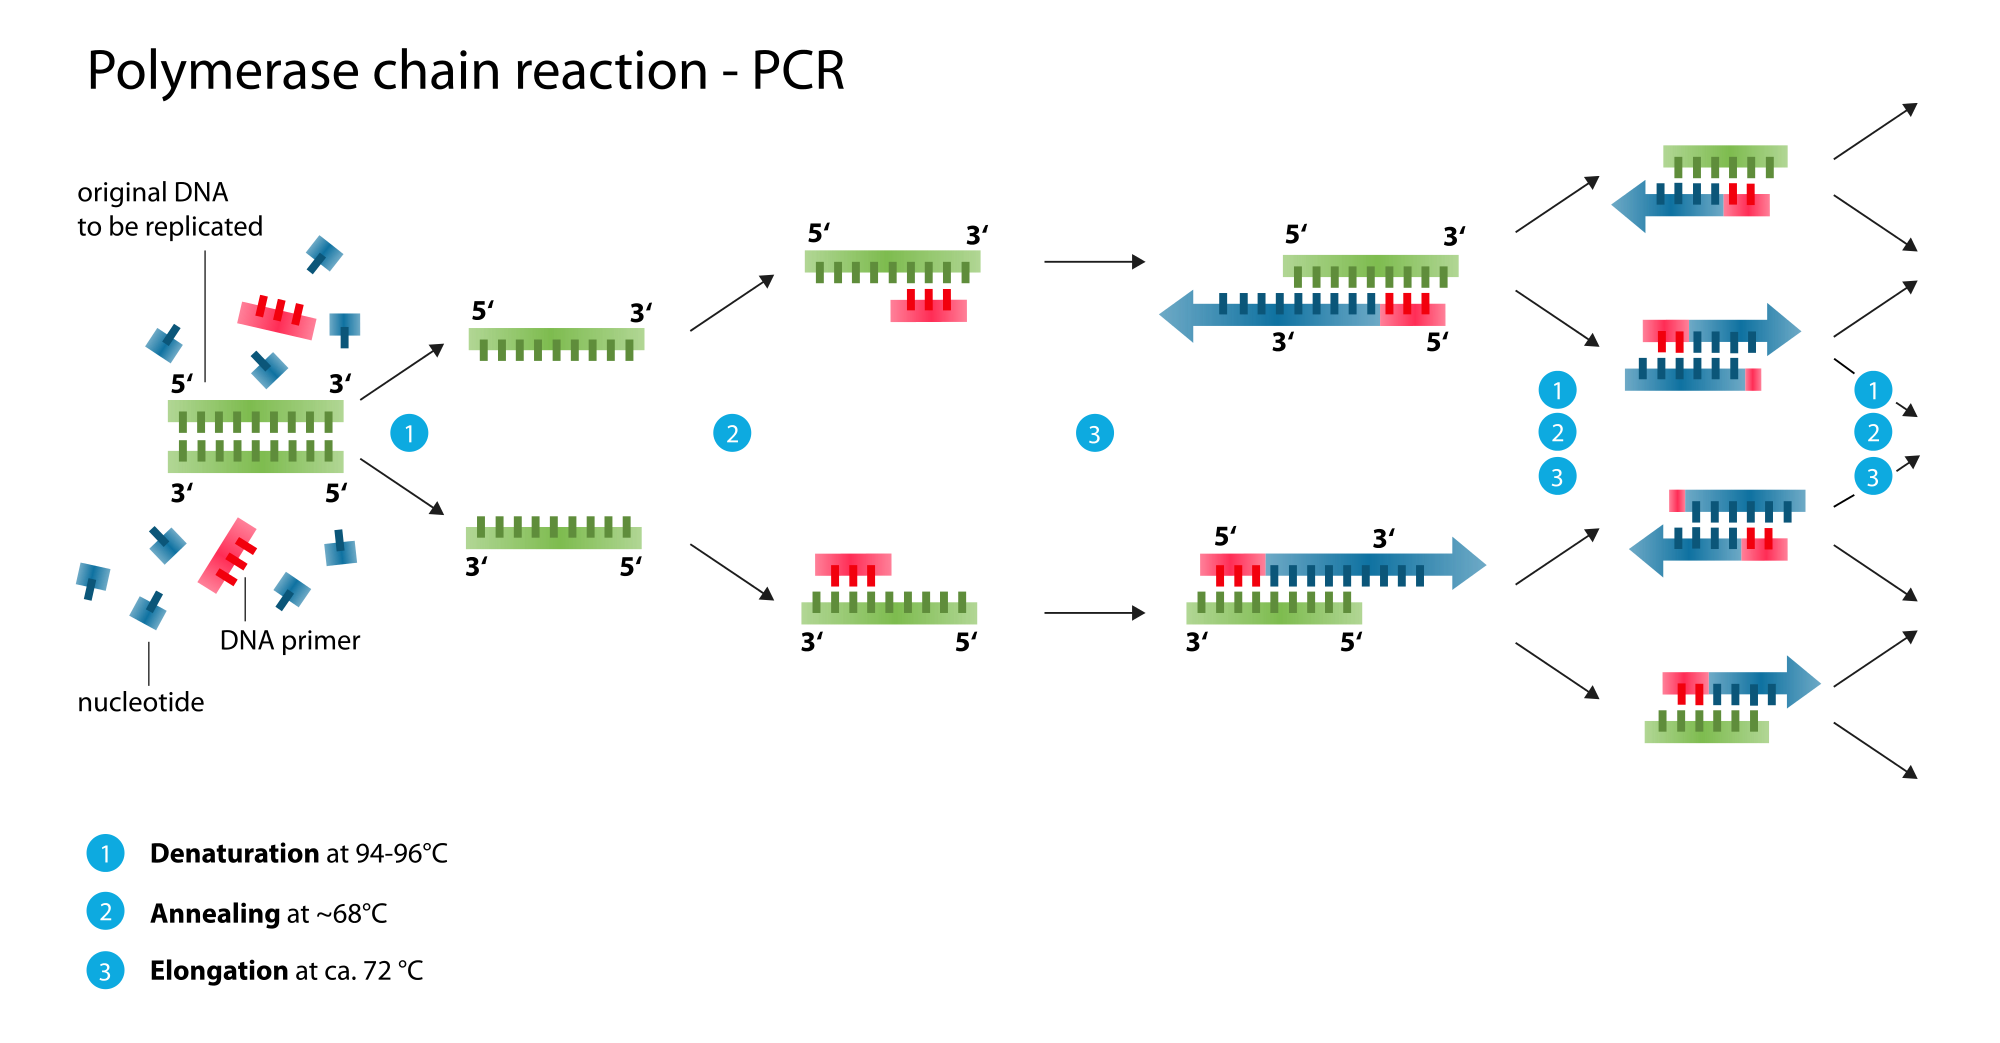
\includegraphics[scale=0.12]{OM-images/pcr_chain.png}}
			\caption{\tiny{Polymerase Chain Reaction (PCR):  Steps, Types, Applications, Microbeonline, 2021}}
		\end{figure}
	\end{column}
	\end{columns}
\end{frame}

\begin{frame}{Low Cost PCR device}
	\begin{columns}
		\begin{column}[T]{0.5\textwidth}
			\vspace*{4ex}
			\begin{itemize}
				\item There has been many efforts on creating Low-Cost PCR device. Most of them only supported low number of reaction chambers (4 to 8) due to their small size.
			\end{itemize}
		\end{column}
		\begin{column}{0.5\textwidth}
			\begin{figure}
				\centering
				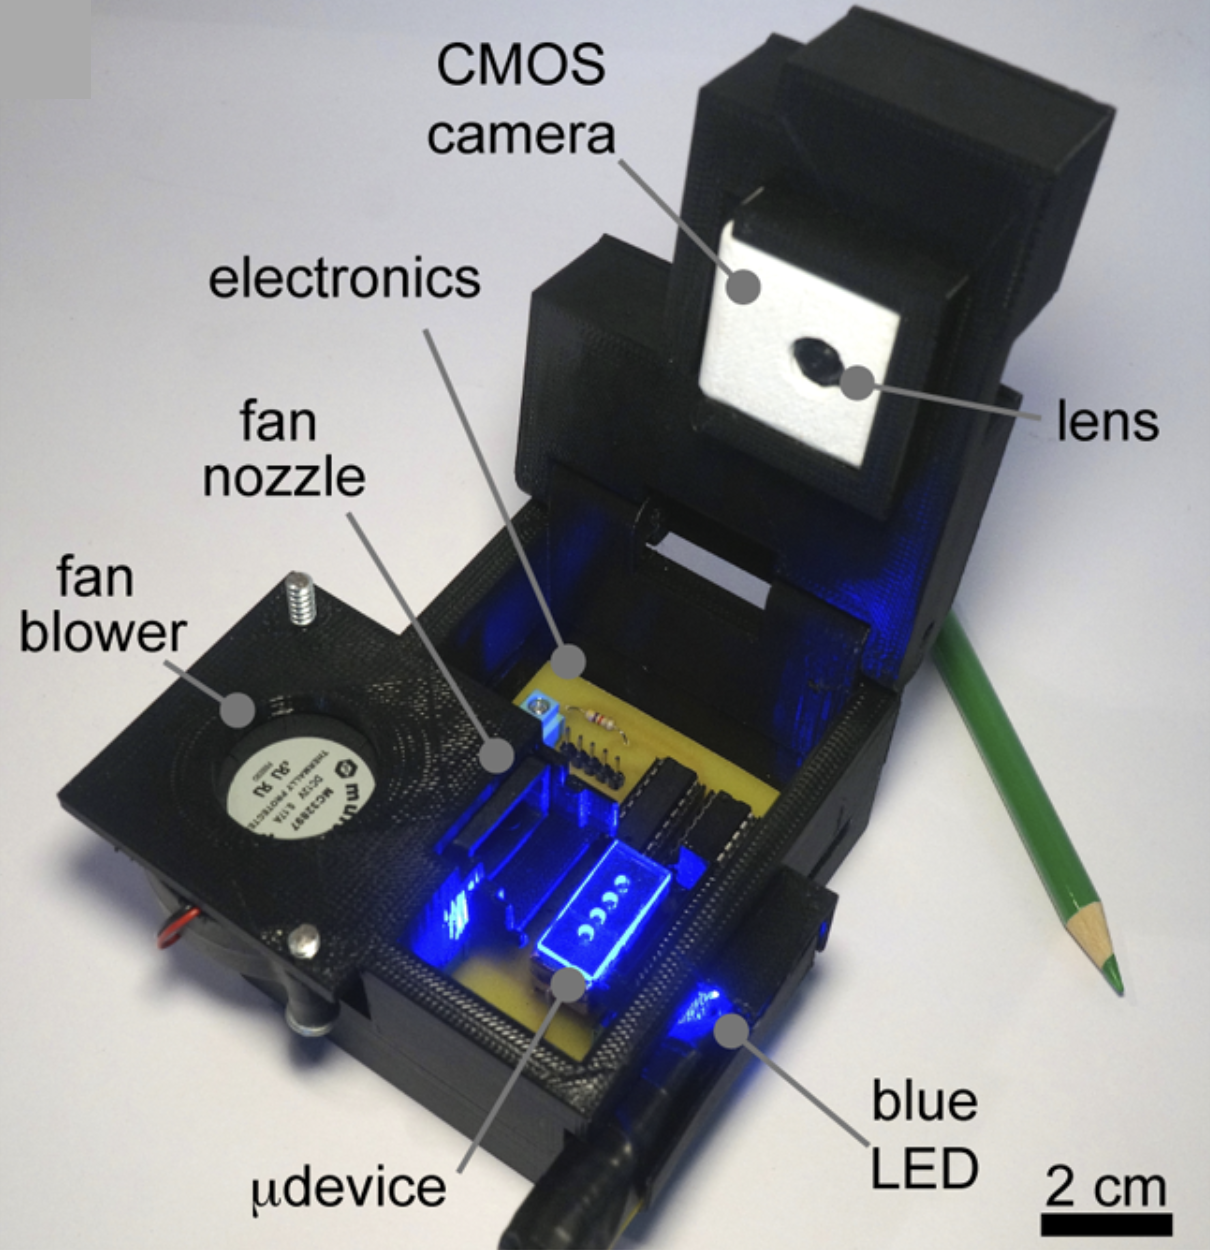
\includegraphics[scale=0.25]{OM-images/pcr1.png}
				\caption{\tiny{Mendoza et al., Analytical Chemistry, 2018}}
			\end{figure}
		\end{column}
	\end{columns}
\end{frame}

\begin{frame}{Low Cost PCR device}
	\begin{columns}
		\begin{column}[T]{0.5\textwidth}
			\vspace*{4ex}
			\begin{itemize}
				\item There have been novel ideas to make it cost even less!
			\end{itemize}
		\end{column}
		\begin{column}{0.5\textwidth}
			\begin{figure}
				\centering
				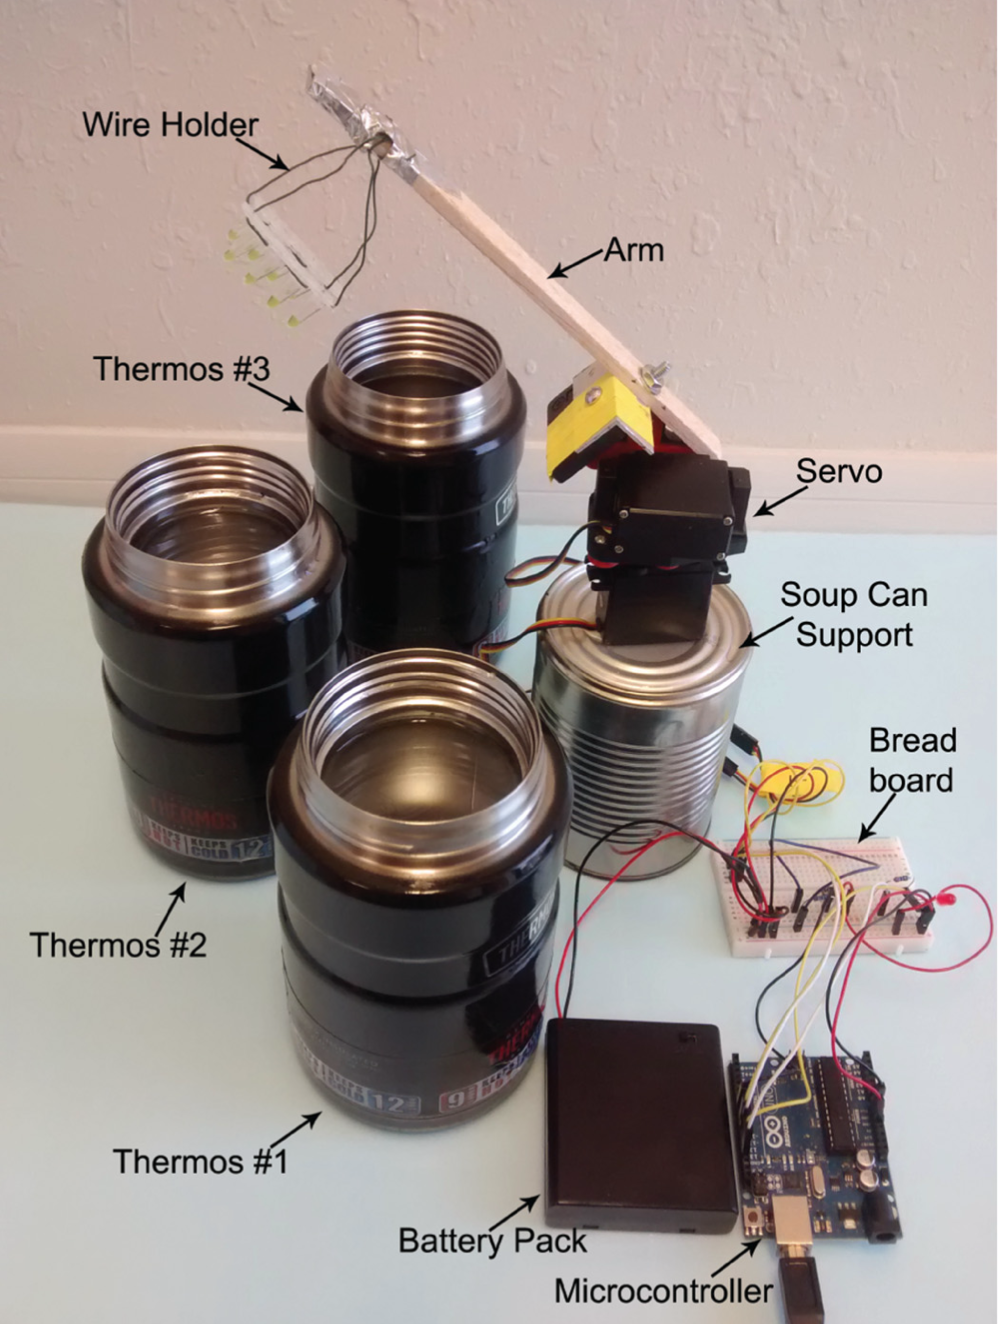
\includegraphics[scale=0.25]{OM-images/pcr2.png}
				\caption{\tiny{Chan et al., Plos One, 2016}}
			\end{figure}
		\end{column}
	\end{columns}
\end{frame}

\begin{frame}{PCR analysis and ML}
	\begin{columns}
		\begin{column}[T]{0.5\textwidth}
			\vspace*{4ex}
			\begin{itemize}
				\item ML has been used for designing the primers, predicting the result of a PCR reaction and etc.
				\item Most of the packages have been written using R programming language
			\end{itemize}
		\end{column}
		\begin{column}{0.5\textwidth}
			\begin{figure}
				\centering
				
\includegraphics[scale=0.45]{OM-images/Rlogo.png}
				\caption{\tiny{}}
			\end{figure}
		\end{column}
	\end{columns}
\end{frame}

\begin{frame}{Future Steps}
	\begin{columns}
		\begin{column}[T]{0.8\textwidth}
			\vspace*{4ex}
			\begin{enumerate}
				\item Completely Implementing the New Optical Subsystem.
				\item Real-Time File Transfer and Processing using Wireless Connections.
				\item Running more tests to obtain data.
				\item Implement ML algorithms to Image Processing and Temperature Control Subsytstems .
			\end{enumerate}
		\end{column}
		\begin{column}{0.2\textwidth}
		\end{column}
	\end{columns}
\end{frame}

\begin{frame}{Conclusion}
	\begin{columns}
		\begin{column}[T]{0.8\textwidth}
			\vspace*{4ex}
			\begin{itemize}
				\item Basics of PCR process was described.
				\item A brief literature review on the subject.
				\item Progress made on Optical Subsystem and Computational Subsystem reported.
				\item Future roadmap explained.
			\end{itemize}
		\end{column}
		\begin{column}{0.2\textwidth}
		\end{column}
	\end{columns}
\end{frame}

\begin{frame}[allowframebreaks]{References}

    \begin{thebibliography}{}

        % Article is the default.
        \bibitem{mendoza}
        Mendoza-Gallegos et al.
        \newblock \emph{An affordable and portable thermocycler for real-time PCR made of 3D-printed parts and off-the-shelf electronics}.
        \newblock  Analytical chemistry, 2018
        
        \bibitem{chan}
        Chan et al.
        \newblock \emph{A Rapid and Low-Cost PCR Thermal Cycler for Infectious Disease Diagnostics}.
        \newblock   PLOS ONE, 2016
        
        \bibitem{nicole}
        Nicole Jawerth
        \newblock \emph{How is the COVID-19 virus detected using real time RT–PCR?}.
        \newblock   IAEA Bulletin, 2020
        
        \bibitem{acharya}
        Acharya Tankeshwar
        \newblock \emph{Polymerase Chain Reaction (PCR):  Steps, Types, Applications}.
        \newblock   Microbe Online, 2021

    \end{thebibliography}
\end{frame}
\end{document}

